\makeheading{2020-03-30}
\section{Colouring and Planar Graphs}
\begin{defbox}
    \begin{definition}
        Let $ G=(V,E) $ be a graph and $ k\in\mathbb{Z}_{\geqslant 1} $.
        A \textbf{\emph{$k$-colouring}} of $ G $ is an assignment of
        `colours' from the set $ \{1,\ldots ,k\} $ to the vertices
        of $ G $ so that the adjacent vertices receive different colours.
    \end{definition}
\end{defbox}

\begin{figure}[H]
    \centering
    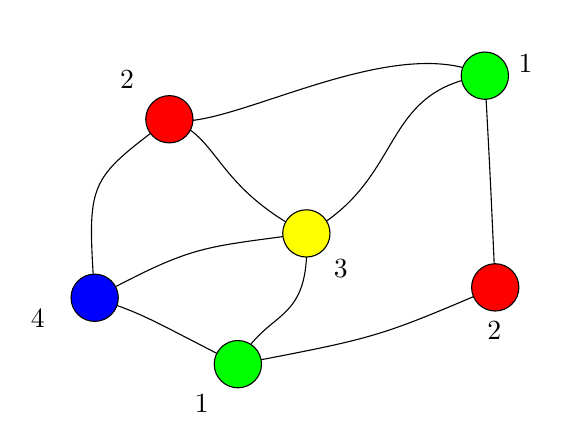
\begin{tikzpicture}[x=0.75pt,y=0.75pt,yscale=-1,xscale=1]
        %uncomment if require: \path (0,300); %set diagram left start at 0, and has height of 300

        %Curve Lines [id:da185009883879945] 
        \draw    (118.38,162.38) .. controls (114.77,105.53) and (114.38,106.38) .. (154.38,76.38) ;
        %Curve Lines [id:da5613565751091367] 
        \draw    (118.38,162.38) .. controls (142.77,170.53) and (142.77,171.53) .. (187.38,194.38) ;
        %Curve Lines [id:da22814701121413616] 
        \draw    (154.38,76.38) .. controls (178.77,84.53) and (175.77,108.53) .. (220.38,131.38) ;
        %Curve Lines [id:da40348870887263244] 
        \draw    (154.38,76.38) .. controls (178.77,84.53) and (261.77,32.53) .. (306.38,55.38) ;
        %Curve Lines [id:da6367573480425464] 
        \draw    (311.38,157.38) .. controls (308.77,98.53) and (308.77,100.53) .. (306.38,55.38) ;
        %Curve Lines [id:da7450601237714736] 
        \draw    (187.38,194.38) .. controls (254.77,181.53) and (254.77,181.53) .. (311.38,157.38) ;
        %Curve Lines [id:da43386596065490957] 
        \draw    (187.38,194.38) .. controls (201.77,166.53) and (222.77,176.53) .. (220.38,131.38) ;
        %Curve Lines [id:da9207283134356746] 
        \draw    (220.38,131.38) .. controls (168.77,138.53) and (166.77,136.53) .. (118.38,162.38) ;
        %Curve Lines [id:da07807249488402457] 
        \draw    (306.38,55.38) .. controls (254.77,62.53) and (268.77,105.53) .. (220.38,131.38) ;
        %Shape: Circle [id:dp3691052451171356] 
        \draw  [fill={rgb, 255:red, 255; green, 0; blue, 0 }  ,fill opacity=1 ] (143,76.38) .. controls (143,70.1) and (148.1,65) .. (154.38,65) .. controls (160.67,65) and (165.77,70.1) .. (165.77,76.38) .. controls (165.77,82.67) and (160.67,87.77) .. (154.38,87.77) .. controls (148.1,87.77) and (143,82.67) .. (143,76.38) -- cycle ;
        %Shape: Circle [id:dp6995325032319567] 
        \draw  [fill={rgb, 255:red, 0; green, 0; blue, 255 }  ,fill opacity=1 ] (107,162.38) .. controls (107,156.1) and (112.1,151) .. (118.38,151) .. controls (124.67,151) and (129.77,156.1) .. (129.77,162.38) .. controls (129.77,168.67) and (124.67,173.77) .. (118.38,173.77) .. controls (112.1,173.77) and (107,168.67) .. (107,162.38) -- cycle ;
        %Shape: Circle [id:dp5936427585593727] 
        \draw  [fill={rgb, 255:red, 255; green, 255; blue, 0 }  ,fill opacity=1 ] (209,131.38) .. controls (209,125.1) and (214.1,120) .. (220.38,120) .. controls (226.67,120) and (231.77,125.1) .. (231.77,131.38) .. controls (231.77,137.67) and (226.67,142.77) .. (220.38,142.77) .. controls (214.1,142.77) and (209,137.67) .. (209,131.38) -- cycle ;
        %Shape: Circle [id:dp9240162309341183] 
        \draw  [fill={rgb, 255:red, 255; green, 0; blue, 0 }  ,fill opacity=1 ] (300,157.38) .. controls (300,151.1) and (305.1,146) .. (311.38,146) .. controls (317.67,146) and (322.77,151.1) .. (322.77,157.38) .. controls (322.77,163.67) and (317.67,168.77) .. (311.38,168.77) .. controls (305.1,168.77) and (300,163.67) .. (300,157.38) -- cycle ;
        %Shape: Circle [id:dp21130823752267514] 
        \draw  [fill={rgb, 255:red, 0; green, 255; blue, 0 }  ,fill opacity=1 ] (295,55.38) .. controls (295,49.1) and (300.1,44) .. (306.38,44) .. controls (312.67,44) and (317.77,49.1) .. (317.77,55.38) .. controls (317.77,61.67) and (312.67,66.77) .. (306.38,66.77) .. controls (300.1,66.77) and (295,61.67) .. (295,55.38) -- cycle ;
        %Shape: Circle [id:dp08386830823435165] 
        \draw  [fill={rgb, 255:red, 0; green, 255; blue, 0 }  ,fill opacity=1 ] (176,194.38) .. controls (176,188.1) and (181.1,183) .. (187.38,183) .. controls (193.67,183) and (198.77,188.1) .. (198.77,194.38) .. controls (198.77,200.67) and (193.67,205.77) .. (187.38,205.77) .. controls (181.1,205.77) and (176,200.67) .. (176,194.38) -- cycle ;

        % Text Node
        \draw (321.38,43.78) node [anchor=north west][inner sep=0.75pt]    {$1$};
        % Text Node
        \draw (306.38,172.78) node [anchor=north west][inner sep=0.75pt]    {$2$};
        % Text Node
        \draw (232.38,142.78) node [anchor=north west][inner sep=0.75pt]    {$3$};
        % Text Node
        \draw (165.38,207.78) node [anchor=north west][inner sep=0.75pt]    {$1$};
        % Text Node
        \draw (86.38,166.78) node [anchor=north west][inner sep=0.75pt]    {$4$};
        % Text Node
        \draw (129.38,51.78) node [anchor=north west][inner sep=0.75pt]    {$2$};
    \end{tikzpicture}
    \caption{$4$-colouring of a graph.}
\end{figure}

\begin{defbox}
    \begin{definition}
        The \textbf{\emph{chromatic number}}, denoted
        $ \chi(G) $, of a graph $ G $ is the minimum
        $ k $ such that $ G $ has a $ k $-colouring.
    \end{definition}
\end{defbox}

\underline{Four-colour problem}: Is it true that every planar graph
has chromatic number $ \leqslant 4 $?

\underline{Answer}: Yes. Appel and Hacken (1977).
The proof was one of the first done with a computer.

\begin{thmbox}
    \begin{lemma}
        Every non-empty planar graph has a vertex of degree $ \leqslant 5 $.
    \end{lemma}
\end{thmbox}
\begin{proof}
    The average degree of a vertex $ v $ of $ G=(V,E) $ is
    \begin{equation*}
        \begin{aligned}
            \frac{1}{|V|} \sum\limits_{v\in V(G)}\deg(v)
             & =\frac{2|E|}{|V|}               & \quad & \text{Handshaking Lemma}   \\
             & \leqslant \frac{2(3|V|-6)}{|V|} & \quad & \text{by~\ref{bound edge}} \\
             & =6-\frac{12}{|V|}
        \end{aligned}
    \end{equation*}
    so some vertex has degree $ \leqslant 6-\frac{12}{|V|} $ and therefore
    $ \leqslant 5 $.
\end{proof}

\begin{thmbox}
    \begin{theorem}[6-colour Theorem]
        Every planar graph is $ 6 $-colourable.
    \end{theorem}
\end{thmbox}
\begin{proof}
    We prove this by induction on the number of vertices. Clearly,
    every graph with $ 1 $ vertex is $ 6 $-colourable. Let $ G $
    be a planar graph on $ n $ vertices, and suppose inductively
    that every planar graph on $ n-1 $ vertices is $ 6 $-colourable.
    Let $ v $ be a vertex of $ G $ whose degree is $ \leqslant 5 $.


    \begin{figure}[H]
        \centering
        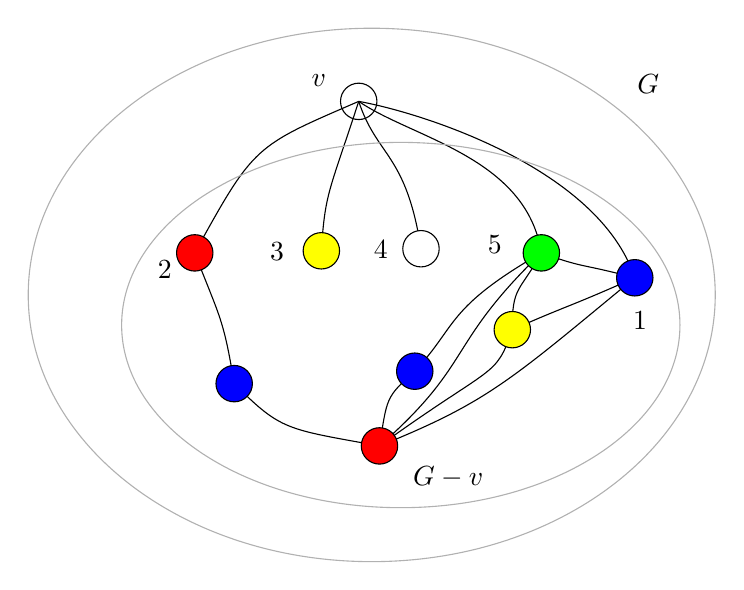
\begin{tikzpicture}[x=0.75pt,y=0.75pt,yscale=-1,xscale=1]
            %uncomment if require: \path (0,300); %set diagram left start at 0, and has height of 300

            %Curve Lines [id:da9712072968440383] 
            \draw    (162,132.77) .. controls (190.77,80.53) and (190.77,81.53) .. (241,59.77) ;
            %Curve Lines [id:da7924097276830756] 
            \draw    (223,131.77) .. controls (224.77,103.53) and (226.77,103.53) .. (241,59.77) ;
            %Curve Lines [id:da9025808851454914] 
            \draw    (271,130.77) .. controls (263.77,84.53) and (249.77,86.53) .. (241,59.77) ;
            %Curve Lines [id:da08194011440733573] 
            \draw    (329,132.77) .. controls (321.77,86.53) and (266.77,77.53) .. (241,59.77) ;
            %Curve Lines [id:da9985145754143169] 
            \draw    (374,144.77) .. controls (356.77,92.53) and (272.77,65.53) .. (241,59.77) ;
            %Curve Lines [id:da15344207278436817] 
            \draw    (315,169.77) .. controls (314.77,148.53) and (318.77,151.53) .. (329,132.77) ;
            %Curve Lines [id:da26355693750326026] 
            \draw    (315,169.77) .. controls (342.77,157.53) and (340.77,159.53) .. (374,144.77) ;
            %Curve Lines [id:da13296377413721794] 
            \draw    (251,225.77) .. controls (303.77,204.53) and (314.77,193.53) .. (374,144.77) ;
            %Curve Lines [id:da9727219365604755] 
            \draw    (181,195.77) .. controls (203.77,218.53) and (205.77,217.53) .. (251,225.77) ;
            %Curve Lines [id:da8243649420730175] 
            \draw    (162,132.77) .. controls (173.77,163.53) and (175.77,163.53) .. (181,195.77) ;
            %Curve Lines [id:da6910598685168583] 
            \draw    (268,189.77) .. controls (288.77,167.53) and (282.77,159.53) .. (329,132.77) ;
            %Curve Lines [id:da461991201657337] 
            \draw    (251,225.77) .. controls (254.77,202.53) and (253.77,202.53) .. (268,189.77) ;
            %Curve Lines [id:da7553080594407117] 
            \draw    (251,225.77) .. controls (306.77,185.53) and (306.77,193.53) .. (315,169.77) ;
            %Curve Lines [id:da5393570855328849] 
            \draw    (251,225.77) .. controls (296.77,185.53) and (282.77,177.53) .. (329,132.77) ;
            %Curve Lines [id:da7869971836410814] 
            \draw    (374,144.77) .. controls (346.77,137.53) and (350.77,140.53) .. (329,132.77) ;
            %Shape: Circle [id:dp03873494285943058] 
            \draw   (232.23,59.77) .. controls (232.23,54.92) and (236.16,51) .. (241,51) .. controls (245.84,51) and (249.77,54.92) .. (249.77,59.77) .. controls (249.77,64.61) and (245.84,68.53) .. (241,68.53) .. controls (236.16,68.53) and (232.23,64.61) .. (232.23,59.77) -- cycle ;
            %Shape: Circle [id:dp859609701497617] 
            \draw  [fill={rgb, 255:red, 255; green, 0; blue, 0 }  ,fill opacity=1 ] (153.23,132.77) .. controls (153.23,127.92) and (157.16,124) .. (162,124) .. controls (166.84,124) and (170.77,127.92) .. (170.77,132.77) .. controls (170.77,137.61) and (166.84,141.53) .. (162,141.53) .. controls (157.16,141.53) and (153.23,137.61) .. (153.23,132.77) -- cycle ;
            %Shape: Circle [id:dp5975902858285127] 
            \draw  [fill={rgb, 255:red, 255; green, 255; blue, 0 }  ,fill opacity=1 ] (214.23,131.77) .. controls (214.23,126.92) and (218.16,123) .. (223,123) .. controls (227.84,123) and (231.77,126.92) .. (231.77,131.77) .. controls (231.77,136.61) and (227.84,140.53) .. (223,140.53) .. controls (218.16,140.53) and (214.23,136.61) .. (214.23,131.77) -- cycle ;
            %Shape: Circle [id:dp06439652328985235] 
            \draw  [fill={rgb, 255:red, 255; green, 255; blue, 255 }  ,fill opacity=1 ] (262.23,130.77) .. controls (262.23,125.92) and (266.16,122) .. (271,122) .. controls (275.84,122) and (279.77,125.92) .. (279.77,130.77) .. controls (279.77,135.61) and (275.84,139.53) .. (271,139.53) .. controls (266.16,139.53) and (262.23,135.61) .. (262.23,130.77) -- cycle ;
            %Shape: Circle [id:dp4510311960366088] 
            \draw  [fill={rgb, 255:red, 0; green, 255; blue, 0 }  ,fill opacity=1 ] (320.23,132.77) .. controls (320.23,127.92) and (324.16,124) .. (329,124) .. controls (333.84,124) and (337.77,127.92) .. (337.77,132.77) .. controls (337.77,137.61) and (333.84,141.53) .. (329,141.53) .. controls (324.16,141.53) and (320.23,137.61) .. (320.23,132.77) -- cycle ;
            %Shape: Circle [id:dp7390141518383276] 
            \draw  [fill={rgb, 255:red, 0; green, 0; blue, 255 }  ,fill opacity=1 ] (365.23,144.77) .. controls (365.23,139.92) and (369.16,136) .. (374,136) .. controls (378.84,136) and (382.77,139.92) .. (382.77,144.77) .. controls (382.77,149.61) and (378.84,153.53) .. (374,153.53) .. controls (369.16,153.53) and (365.23,149.61) .. (365.23,144.77) -- cycle ;
            %Shape: Circle [id:dp42057428227763005] 
            \draw  [fill={rgb, 255:red, 255; green, 255; blue, 0 }  ,fill opacity=1 ] (306.23,169.77) .. controls (306.23,164.92) and (310.16,161) .. (315,161) .. controls (319.84,161) and (323.77,164.92) .. (323.77,169.77) .. controls (323.77,174.61) and (319.84,178.53) .. (315,178.53) .. controls (310.16,178.53) and (306.23,174.61) .. (306.23,169.77) -- cycle ;
            %Shape: Circle [id:dp25709656677230097] 
            \draw  [fill={rgb, 255:red, 0; green, 0; blue, 255 }  ,fill opacity=1 ] (259.23,189.77) .. controls (259.23,184.92) and (263.16,181) .. (268,181) .. controls (272.84,181) and (276.77,184.92) .. (276.77,189.77) .. controls (276.77,194.61) and (272.84,198.53) .. (268,198.53) .. controls (263.16,198.53) and (259.23,194.61) .. (259.23,189.77) -- cycle ;
            %Shape: Circle [id:dp096417586424565] 
            \draw  [fill={rgb, 255:red, 255; green, 0; blue, 0 }  ,fill opacity=1 ] (242.23,225.77) .. controls (242.23,220.92) and (246.16,217) .. (251,217) .. controls (255.84,217) and (259.77,220.92) .. (259.77,225.77) .. controls (259.77,230.61) and (255.84,234.53) .. (251,234.53) .. controls (246.16,234.53) and (242.23,230.61) .. (242.23,225.77) -- cycle ;
            %Shape: Circle [id:dp526272776764649] 
            \draw  [fill={rgb, 255:red, 0; green, 0; blue, 255 }  ,fill opacity=1 ] (172.23,195.77) .. controls (172.23,190.92) and (176.16,187) .. (181,187) .. controls (185.84,187) and (189.77,190.92) .. (189.77,195.77) .. controls (189.77,200.61) and (185.84,204.53) .. (181,204.53) .. controls (176.16,204.53) and (172.23,200.61) .. (172.23,195.77) -- cycle ;
            %Shape: Ellipse [id:dp5462024310027918] 
            \draw  [color={rgb, 255:red, 177; green, 177; blue, 177 }  ,draw opacity=1 ] (126.77,167.53) .. controls (126.77,118.93) and (186.98,79.53) .. (261.27,79.53) .. controls (335.55,79.53) and (395.77,118.93) .. (395.77,167.53) .. controls (395.77,216.13) and (335.55,255.53) .. (261.27,255.53) .. controls (186.98,255.53) and (126.77,216.13) .. (126.77,167.53) -- cycle ;
            %Shape: Ellipse [id:dp9805815600694171] 
            \draw  [color={rgb, 255:red, 177; green, 177; blue, 177 }  ,draw opacity=1 ] (81.77,153.03) .. controls (81.77,82.06) and (155.86,24.53) .. (247.27,24.53) .. controls (338.67,24.53) and (412.77,82.06) .. (412.77,153.03) .. controls (412.77,224) and (338.67,281.53) .. (247.27,281.53) .. controls (155.86,281.53) and (81.77,224) .. (81.77,153.03) -- cycle ;

            % Text Node
            \draw (143,135.4) node [anchor=north west][inner sep=0.75pt]    {$2$};
            % Text Node
            \draw (197,126.4) node [anchor=north west][inner sep=0.75pt]    {$3$};
            % Text Node
            \draw (247,125.4) node [anchor=north west][inner sep=0.75pt]    {$4$};
            % Text Node
            \draw (302,123.4) node [anchor=north west][inner sep=0.75pt]    {$5$};
            % Text Node
            \draw (372,160) node [anchor=north west][inner sep=0.75pt]    {$1$};
            % Text Node
            \draw (374,45.4) node [anchor=north west][inner sep=0.75pt]    {$G$};
            % Text Node
            \draw (266,234.4) node [anchor=north west][inner sep=0.75pt]    {$G-v$};
            % Text Node
            \draw (217,45.4) node [anchor=north west][inner sep=0.75pt]    {$v$};
        \end{tikzpicture}
    \end{figure}

    Inductively, a planar graph $ G-v $ is $ 6 $-colourable. Since
    $ v $ has at most $ 5 $ neighbours, there is a colour
    in $ \{1,2,3,4,5,6\} $ not assigned to any neighbour of $ v $ in $ G $.
    Assigning this colour to $ v $ gives a $ 6 $-colouring of $ G $.
\end{proof}

\begin{thmbox}
    \begin{theorem}[Five-colour Theorem]
        Every planar graph is $ 5 $-colourable.
    \end{theorem}
\end{thmbox}
\begin{proof}
    Induction on $ |V(G)| $. Let $ G $ be a graph on $ n\geqslant 1 $
    vertices and suppose the theorem holds for every planar graph
    $ n-1 $ vertices. Let $ v $ be a vertex of degree $ \leqslant 5 $
    in $ G $. Inductively, $ G-v $ has a $ 5 $-colouring.
    If at most $ 4 $ colours are assigned to neighbours of $ v $,
    then we can extend the colouring of $ G-v $ to a colouring of
    $ G $ by choosing a colour for $ v $ not appearing on
    neighbours of $ v $. Otherwise, there are $ \geqslant 5 $ colours
    appearing on neighbours of $ v $. Since $ v $ has $ \leqslant 5 $
    neighbours, this means every neighbour of $ v $ is assigned
    a different colour.
    Let
    \[ B,\,P,\,G,\,Y,\,W \]
    be the colours occurring on the neighbours of $ v $ as they appear in
    clockwise order around $ v $.

    \begin{figure}[H]
        \centering
        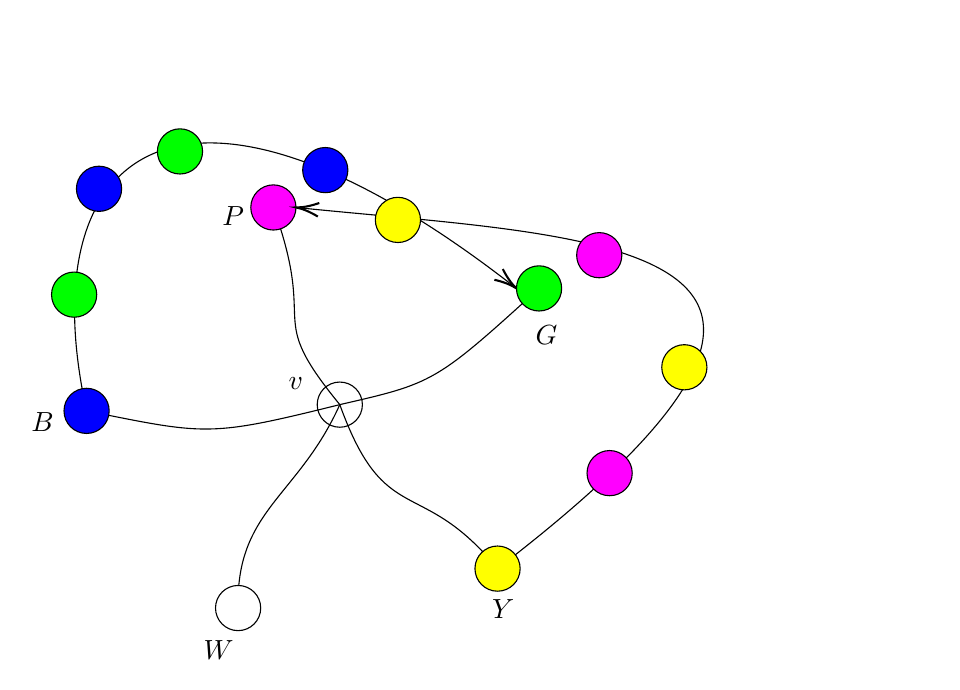
\begin{tikzpicture}[x=0.75pt,y=0.75pt,yscale=-1,xscale=1]
            %uncomment if require: \path (0,300); %set diagram left start at 0, and has height of 300

            %Shape: Circle [id:dp4797712322288732] 
            \draw   (342,134.88) .. controls (342,128.87) and (346.87,124) .. (352.88,124) .. controls (358.89,124) and (363.77,128.87) .. (363.77,134.88) .. controls (363.77,140.89) and (358.89,145.77) .. (352.88,145.77) .. controls (346.87,145.77) and (342,140.89) .. (342,134.88) -- cycle ;
            %Curve Lines [id:da8796410007105212] 
            \draw    (230.88,137.88) .. controls (288.77,149.53) and (289.77,150.53) .. (352.88,134.88) ;
            %Curve Lines [id:da6726897158881784] 
            \draw    (352.88,134.88) .. controls (397.77,124.53) and (398.77,124.53) .. (448.88,78.88) ;
            %Curve Lines [id:da8125629887732329] 
            \draw    (352.88,134.88) .. controls (315.77,89.53) and (342.77,100.53) .. (320.88,39.88) ;
            %Curve Lines [id:da7228080539652716] 
            \draw    (428.88,213.88) .. controls (391.77,168.53) and (374.77,195.53) .. (352.88,134.88) ;
            %Curve Lines [id:da6140567726193096] 
            \draw    (303.88,232.88) .. controls (302.77,185.53) and (332.77,179.53) .. (352.88,134.88) ;
            %Curve Lines [id:da05589707271707145] 
            \draw    (230.88,137.88) .. controls (202.77,10.53) and (277.77,-46.47) .. (438,78.88) ;
            \draw [shift={(438,78.88)}, rotate = 218.04] [color={rgb, 255:red, 0; green, 0; blue, 0 }  ][line width=0.75]    (10.93,-3.29) .. controls (6.95,-1.4) and (3.31,-0.3) .. (0,0) .. controls (3.31,0.3) and (6.95,1.4) .. (10.93,3.29)   ;
            %Shape: Circle [id:dp5045271386500565] 
            \draw  [color={rgb, 255:red, 0; green, 0; blue, 0 }  ,draw opacity=1 ][fill={rgb, 255:red, 0; green, 0; blue, 255 }  ,fill opacity=1 ] (220,137.88) .. controls (220,131.87) and (224.87,127) .. (230.88,127) .. controls (236.89,127) and (241.77,131.87) .. (241.77,137.88) .. controls (241.77,143.89) and (236.89,148.77) .. (230.88,148.77) .. controls (224.87,148.77) and (220,143.89) .. (220,137.88) -- cycle ;
            %Shape: Circle [id:dp6547159764026466] 
            \draw  [color={rgb, 255:red, 0; green, 0; blue, 0 }  ,draw opacity=1 ][fill={rgb, 255:red, 0; green, 0; blue, 255 }  ,fill opacity=1 ] (226,30.88) .. controls (226,24.87) and (230.87,20) .. (236.88,20) .. controls (242.89,20) and (247.77,24.87) .. (247.77,30.88) .. controls (247.77,36.89) and (242.89,41.77) .. (236.88,41.77) .. controls (230.87,41.77) and (226,36.89) .. (226,30.88) -- cycle ;
            %Shape: Circle [id:dp35574065586535086] 
            \draw  [color={rgb, 255:red, 0; green, 0; blue, 0 }  ,draw opacity=1 ][fill={rgb, 255:red, 0; green, 0; blue, 255 }  ,fill opacity=1 ] (335,21.88) .. controls (335,15.87) and (339.87,11) .. (345.88,11) .. controls (351.89,11) and (356.77,15.87) .. (356.77,21.88) .. controls (356.77,27.89) and (351.89,32.77) .. (345.88,32.77) .. controls (339.87,32.77) and (335,27.89) .. (335,21.88) -- cycle ;
            %Shape: Circle [id:dp9695607602451499] 
            \draw  [color={rgb, 255:red, 0; green, 0; blue, 0 }  ,draw opacity=1 ][fill={rgb, 255:red, 255; green, 255; blue, 255 }  ,fill opacity=1 ] (293,232.88) .. controls (293,226.87) and (297.87,222) .. (303.88,222) .. controls (309.89,222) and (314.77,226.87) .. (314.77,232.88) .. controls (314.77,238.89) and (309.89,243.77) .. (303.88,243.77) .. controls (297.87,243.77) and (293,238.89) .. (293,232.88) -- cycle ;
            %Shape: Circle [id:dp40884316891883343] 
            \draw  [color={rgb, 255:red, 0; green, 0; blue, 0 }  ,draw opacity=1 ][fill={rgb, 255:red, 255; green, 0; blue, 255 }  ,fill opacity=1 ] (310,39.88) .. controls (310,33.87) and (314.87,29) .. (320.88,29) .. controls (326.89,29) and (331.77,33.87) .. (331.77,39.88) .. controls (331.77,45.89) and (326.89,50.77) .. (320.88,50.77) .. controls (314.87,50.77) and (310,45.89) .. (310,39.88) -- cycle ;
            %Shape: Circle [id:dp9387122738620363] 
            \draw  [color={rgb, 255:red, 0; green, 0; blue, 0 }  ,draw opacity=1 ][fill={rgb, 255:red, 0; green, 255; blue, 0 }  ,fill opacity=1 ] (438,78.88) .. controls (438,72.87) and (442.87,68) .. (448.88,68) .. controls (454.89,68) and (459.77,72.87) .. (459.77,78.88) .. controls (459.77,84.89) and (454.89,89.77) .. (448.88,89.77) .. controls (442.87,89.77) and (438,84.89) .. (438,78.88) -- cycle ;
            %Shape: Circle [id:dp8179616541550487] 
            \draw  [color={rgb, 255:red, 0; green, 0; blue, 0 }  ,draw opacity=1 ][fill={rgb, 255:red, 0; green, 255; blue, 0 }  ,fill opacity=1 ] (214,81.88) .. controls (214,75.87) and (218.87,71) .. (224.88,71) .. controls (230.89,71) and (235.77,75.87) .. (235.77,81.88) .. controls (235.77,87.89) and (230.89,92.77) .. (224.88,92.77) .. controls (218.87,92.77) and (214,87.89) .. (214,81.88) -- cycle ;
            %Shape: Circle [id:dp9047411695715875] 
            \draw  [color={rgb, 255:red, 0; green, 0; blue, 0 }  ,draw opacity=1 ][fill={rgb, 255:red, 0; green, 255; blue, 0 }  ,fill opacity=1 ] (265,12.88) .. controls (265,6.87) and (269.87,2) .. (275.88,2) .. controls (281.89,2) and (286.77,6.87) .. (286.77,12.88) .. controls (286.77,18.89) and (281.89,23.77) .. (275.88,23.77) .. controls (269.87,23.77) and (265,18.89) .. (265,12.88) -- cycle ;
            %Curve Lines [id:da021574929102323392] 
            \draw    (428.88,213.88) .. controls (637.77,53.53) and (473.65,54.53) .. (331.77,39.88) ;
            \draw [shift={(331.77,39.88)}, rotate = 365.9] [color={rgb, 255:red, 0; green, 0; blue, 0 }  ][line width=0.75]    (10.93,-3.29) .. controls (6.95,-1.4) and (3.31,-0.3) .. (0,0) .. controls (3.31,0.3) and (6.95,1.4) .. (10.93,3.29)   ;
            %Shape: Circle [id:dp6822555424394983] 
            \draw  [color={rgb, 255:red, 0; green, 0; blue, 0 }  ,draw opacity=1 ][fill={rgb, 255:red, 255; green, 255; blue, 0 }  ,fill opacity=1 ] (418,213.88) .. controls (418,207.87) and (422.87,203) .. (428.88,203) .. controls (434.89,203) and (439.77,207.87) .. (439.77,213.88) .. controls (439.77,219.89) and (434.89,224.77) .. (428.88,224.77) .. controls (422.87,224.77) and (418,219.89) .. (418,213.88) -- cycle ;
            %Shape: Circle [id:dp2753561318647072] 
            \draw  [color={rgb, 255:red, 0; green, 0; blue, 0 }  ,draw opacity=1 ][fill={rgb, 255:red, 255; green, 0; blue, 255 }  ,fill opacity=1 ] (472,167.88) .. controls (472,161.87) and (476.87,157) .. (482.88,157) .. controls (488.89,157) and (493.77,161.87) .. (493.77,167.88) .. controls (493.77,173.89) and (488.89,178.77) .. (482.88,178.77) .. controls (476.87,178.77) and (472,173.89) .. (472,167.88) -- cycle ;
            %Shape: Circle [id:dp46764582752573225] 
            \draw  [color={rgb, 255:red, 0; green, 0; blue, 0 }  ,draw opacity=1 ][fill={rgb, 255:red, 255; green, 0; blue, 255 }  ,fill opacity=1 ] (467,62.88) .. controls (467,56.87) and (471.87,52) .. (477.88,52) .. controls (483.89,52) and (488.77,56.87) .. (488.77,62.88) .. controls (488.77,68.89) and (483.89,73.77) .. (477.88,73.77) .. controls (471.87,73.77) and (467,68.89) .. (467,62.88) -- cycle ;
            %Shape: Circle [id:dp33066797329649555] 
            \draw  [color={rgb, 255:red, 0; green, 0; blue, 0 }  ,draw opacity=1 ][fill={rgb, 255:red, 255; green, 255; blue, 0 }  ,fill opacity=1 ] (508,116.88) .. controls (508,110.87) and (512.87,106) .. (518.88,106) .. controls (524.89,106) and (529.77,110.87) .. (529.77,116.88) .. controls (529.77,122.89) and (524.89,127.77) .. (518.88,127.77) .. controls (512.87,127.77) and (508,122.89) .. (508,116.88) -- cycle ;
            %Shape: Circle [id:dp8258844104040124] 
            \draw  [color={rgb, 255:red, 0; green, 0; blue, 0 }  ,draw opacity=1 ][fill={rgb, 255:red, 255; green, 255; blue, 0 }  ,fill opacity=1 ] (370,45.88) .. controls (370,39.87) and (374.87,35) .. (380.88,35) .. controls (386.89,35) and (391.77,39.87) .. (391.77,45.88) .. controls (391.77,51.89) and (386.89,56.77) .. (380.88,56.77) .. controls (374.87,56.77) and (370,51.89) .. (370,45.88) -- cycle ;

            % Text Node
            \draw (327,120.4) node [anchor=north west][inner sep=0.75pt]    {$v$};
            % Text Node
            \draw (203,137.4) node [anchor=north west][inner sep=0.75pt]    {$B$};
            % Text Node
            \draw (295,38.4) node [anchor=north west][inner sep=0.75pt]    {$P$};
            % Text Node
            \draw (446,95.4) node [anchor=north west][inner sep=0.75pt]    {$G$};
            % Text Node
            \draw (425,227.4) node [anchor=north west][inner sep=0.75pt]    {$Y$};
            % Text Node
            \draw (286,247.4) node [anchor=north west][inner sep=0.75pt]    {$W$};

        \end{tikzpicture}

    \end{figure}

    Let $ G_{GB} $ be the subgraph
    of $ G-v $ induced by the green and blue vertices. Define $ G_{PY} $
    similarly. By the planarity of $ G $, either the $ G,B $
    neighbours of $ v $ are disconnected in $ G_{GB} $, or the $ P,Y $
    neighbours of $ v $ are disconnected in $ G_{PY} $. Suppose by
    symmetry the first case holds.

    Let $ u,w $ be the $ B,G $ neighbours of $ v $ so $ u,w $ are disconnected
    in $ G_{GB} $. Let $ C $ be the component of $ G_{GB} $ containing
    $ u $. Now, form a new $ 5 $-colouring of $ G-v $ by switching
    the colour of every vertex of $ C $ from $ G $ to $ B $ or vice versa.
    This gives a $ 5 $-colouring of $ G-v $ in which both $ u $ and $ w $
    are $ G $ (because $ w\notin C $). Now, we can colour $ v $
    blue to get a $ 5 $-colouring of $ G $.
\end{proof}
